\documentclass[12pt,letterpaper]{article}

\usepackage[T1]{fontenc}
\usepackage[margin=0.75in,headheight=1.5em]{geometry}
\usepackage{enumitem}
\usepackage{fancyhdr}
\usepackage{lastpage}
\usepackage{float}
\usepackage{tabu}
\usepackage{booktabs}
\usepackage{graphicx}
\usepackage{lmodern}
\usepackage[table]{xcolor}  
\usepackage[font=bf]{caption}

\begin{document}

\renewcommand\headrule{}

\pagestyle{fancy}
\fancyhf{}
\lfoot{COMP 3004}
\rfoot{\thepage/\pageref{LastPage}}
\cfoot{System Design Document}

% CUSTOM COMMANDS
\newcommand{\twodigits}[1]{\ifnum\value{#1}<10 0\fi\arabic{#1}}

\newcommand{\teamname}{Code First, Think Later}
\newcommand{\personone}{Kevin Hua}
\newcommand{\persontwo}{Hendrik Knoetze}
\newcommand{\personthree}{Juhandr\'e Knoetze}

%% FIGURE COMMANDS
\newcommand{\figurelabel}[1]{\label{figure:#1}}
\newcommand{\figureref}[1]{\textbf{Figure \ref{figure:#1}}}
%% END FIGURE COMMANDS

%% TABLE COMMANDS
\definecolor{thcolor}{RGB}{193,193,193}
\newcommand{\ccindent}{\hspace{1.5em}\hangindent=1.5em}
\newcommand{\tableheader}{\rowfont\bf\rowcolor{thcolor!30}}

\newcommand{\tablelabel}[1]{\label{table:#1}}
\newcommand{\tableref}[1]{\textbf{Table \ref{table:#1}}}
%% END TABLE COMMANDS

%% NODE COMMANDS
\newcounter{nodenum}
\renewcommand{\thenodenum}{\twodigits{nodenum}}
\newcommand{\nlabel}[1]{\refstepcounter{nodenum}\label{n:#1}}
\newcommand{\nref}[1]{\textbf{N-\ref{n:#1}}}
%% END NODE COMMANDS

%% SUBSYSTEM COMMANDS
\newcounter{subsystemnum}
\renewcommand{\thesubsystemnum}{\twodigits{subsystemnum}}
\newcommand{\sdlabel}[1]{\refstepcounter{subsystemnum}\label{sd:#1}}
\newcommand{\sdref}[1]{\textbf{SD-\ref{sd:#1}}}
%% END SUBSYSTEM COMMANDS

%% CLASS DIAGRAM COMMANDS
\newcounter{classdiagramnum}
\renewcommand{\theclassdiagramnum}{\twodigits{classdiagramnum}}
\newcommand{\cdlabel}[1]{\refstepcounter{classdiagramnum}\label{cd:#1}}
\newcommand{\cdref}[1]{\textbf{CD-\ref{cd:#1}}}
%% END CLASS DIAGRAM COMMANDS

%% DESIGN PATTERNS COMMANDS
\newcounter{designpatternnum}
\renewcommand{\thedesignpatternnum}{\twodigits{designpatternnum}}
\newcommand{\dplabel}[1]{\refstepcounter{designpatternnum}\label{dp:#1}}
\newcommand{\dpref}[1]{\textbf{DP-\ref{dp:#1}}}
%% END DESIGN PATTERNS COMMANDS

%% SERVICES COMMANDS
\newcounter{servicenum}
\renewcommand{\theservicenum}{\twodigits{servicenum}}
\newcommand{\sslabel}[1]{\refstepcounter{servicenum}\label{ss:#1}}
\newcommand{\ssref}[1]{\textbf{SS-\ref{ss:#1}}}
%% END SERVICES COMMANDS

%% OPERATIONS COMMANDS
\newcounter{operationnum}
\renewcommand{\theoperationnum}{\twodigits{operationnum}}
\newcommand{\oplabel}[1]{\refstepcounter{operationnum}\label{op:#1}}
\newcommand{\opref}[1]{\textbf{OP-\ref{op:#1}}}
%% END OPERATIONS COMMANDS

%% TABLE COMMANDS
\newcounter{dbtablenum}
\renewcommand{\thedbtablenum}{\twodigits{dbtablenum}}
\newcommand{\dtlabel}[1]{\refstepcounter{dbtablenum}\label{dt:#1}}
\newcommand{\dtref}[1]{\textbf{DT-\ref{dt:#1}}}
%% END TABLE COMMANDS

% TABLE STYLING
\everyrow{\hline}
\tabulinesep=0.5em

\setlist[itemize]{leftmargin=*,noitemsep,nolistsep}
\setlist[enumerate]{leftmargin=*,noitemsep,nolistsep}
% END TABLE STYLING

\thispagestyle{empty}

\begin{center}
	CARLETON UNIVERSITY
\end{center}

\vfill

\begin{center}
	{\fontsize{55pt}{55pt}\selectfont cuPID}
	\vspace{0.5em}\rule{\textwidth}{0.5pt}
	System Design Document
\end{center}

\vspace{5em}

\begin{center}
	\textbf{Team [\teamname{}]}\\
	\personone{}\\
	\persontwo{}\\
	\personthree{}
\end{center}

\vfill

\begin{center}
	Submitted to:\\
	Dr. Christine Laurendeau\\
	COMP 3004: Object Oriented Software Engineering\\
	School of Computer Science\\
	Carleton University
\end{center}

\vspace{2em}

\begin{center}
	\today
\end{center}

\newpage{}

\tableofcontents{}

\renewcommand{\listfigurename}{Figures}
\listoffigures

\renewcommand{\listtablename}{Tables}
\listoftables

\newpage{}

\section{Introduction}

\subsection{Purpose of System}

Team projects are intrinsically part of every student's academic life at some point or another. Many become resigned to losing the marks due to poor compatbility with assigned team members. This system has been designed to alleviate some of that pain by removing both the random factor and human error with regards to an educator's decision. Our system employs a special sorting algorithm that we have developed that combines psychological knowledge and research with computational reliability.

 Loosely speaking, the purpose of this system is to sort a group or class of people into groups of a specified size. However, more than just sorting people, our software takes into account a total of fifteen different characteristics of a person to determine the most optimal team that is based on more than just academic achievement. Here at [Code First, Think Later], we strongly believe that smart people don't have to like another smart person simply because they're smart.

\subsection{Overview of Document}

This report will provide an updated overview of various design decisions with regards to our system. This new system aims to correct all the shortcomings of the previous prototype, as well as smooth out several other issues that we encountered during the coding of the prototype. Futhermore, at this stage of development, it is time to revise and reorganize our prototype in such a way that it adheres more closely with both a reliable architectural style and appropriate design styles. 

Beginning with a full decomposition of our prototype, we will then show a modified decomposition wherein poor design choices have been fixed. Following these decompositions, our report will feature our chosen strategies with regards to architectural and design styles. We will also be covering the details of our persistent storage system in this section. Afterwards, we will revisit the subsystems that we have decomposed in the first section and provide a detailed set of descriptions as to what services each offers in the grand scheme of things. Finally, we will end the report with a UML style set of class diagrams for each class.

\vspace{1em}

\noindent Best regards,

\vspace{1em}

\begin{center}
	
\includegraphics[scale=0.4]{imgs/logo.png} \\ \footnotesize{(Team [Code First, Think Later])}
\end{center}

\section{Subsystem Decomposition}

This section will be three-pronged - firstly, we will decompose the current working prototype into its corresponding set of logical subsystem. Following, we will introduce a more complete system decomposition, wherein we will include aspects that are not yet implemented in the current cuPID prototype. Also in this part, we will possibly modify existing subsystmes from the prototype to promote a higher degree of cohesion and minimal coupling. Finally, we will discuss the changes that we have decided on and how they impact the software as a whole. 

\subsection{Phase 1 Prototype Decomposition}
\begin{figure}[H]
	\centering{}
	\includegraphics[scale=0.55]{imgs/d3/class-diagram-prototype.png}
	\caption{Subsystem Decomposition (Prototype)}
	\figurelabel{proto-decomp}
\end{figure}
\subsection{System Decomposition}
\begin{figure}[H]
	\centering{}
	\includegraphics[scale=0.3]{imgs/d3/class-diagram-decomp.png}
	\caption{Subsystem Decomposition}
	\figurelabel{subsys-decomp}
\end{figure}
\subsection{Design Evolution}
\subsubsection{Prototype Design Decisions}
\subsubsection{Updated Design Decisions}
\section{Design Strategies}

Similar to the previous section, this section is also divided into three major parts: architectural style, persistent data management, and design patterns. In the first part, we will describe our chosen architectural style and explain the benefits to using this particular style with regards to our system. We will also include UML deployment diagrams as a visual representation of the architecture of our software. Following this part, we will discuss our design choices with regards to our persistent data management. We will also be covering some particular cases here, such as duplicate records. Finally, we will discuss the our chosen design patterns and why they are appropriate given our decisions form the other parts in this section.

\subsection{Hardware/Software Mapping}
\subsubsection{Overview}

Our system revolves heavily upon a central storage, or repository. Other than the repository, we make use of several subsystems. Simply with this in mind, we can instantly rule out the {\it pipe and filter} architectural style - while we do indeed have subsystems (filters) that associate with each other (pipes), our subsystems are fairly dependent on one another. Furthermore, our subsystems are responsible for more than simply processing a set of inputs to get a set of outputs. 

We can also rule out the four-tier architectural style right away - our system is entirely local, thus a separate client and server layer are unnecessary. We use a login-type system, and the UI is common to any user that logs in. The only difference would be that the displayed information changes, as well as some usability. That said, this type of functionality would best fit as multiple partitions within a layer. As a result, the difference in the student and admin users should be as sister partitions within the same layer.

\subsubsection{Three-Tier Architecture}

Three-tier architecture involves dividing the system into three layers - the interface layer, the logic layer, and the storage layer. While it is more than possible, and, indeed, even appealing to consider such a decomposition, we decided not to go with this style. Unfortunately, this style, while having fairly high cohesion, has equally high coupling. For these reasons, we have decided to discard this architectural style.

\begin{figure}[H]
	\centering{}
	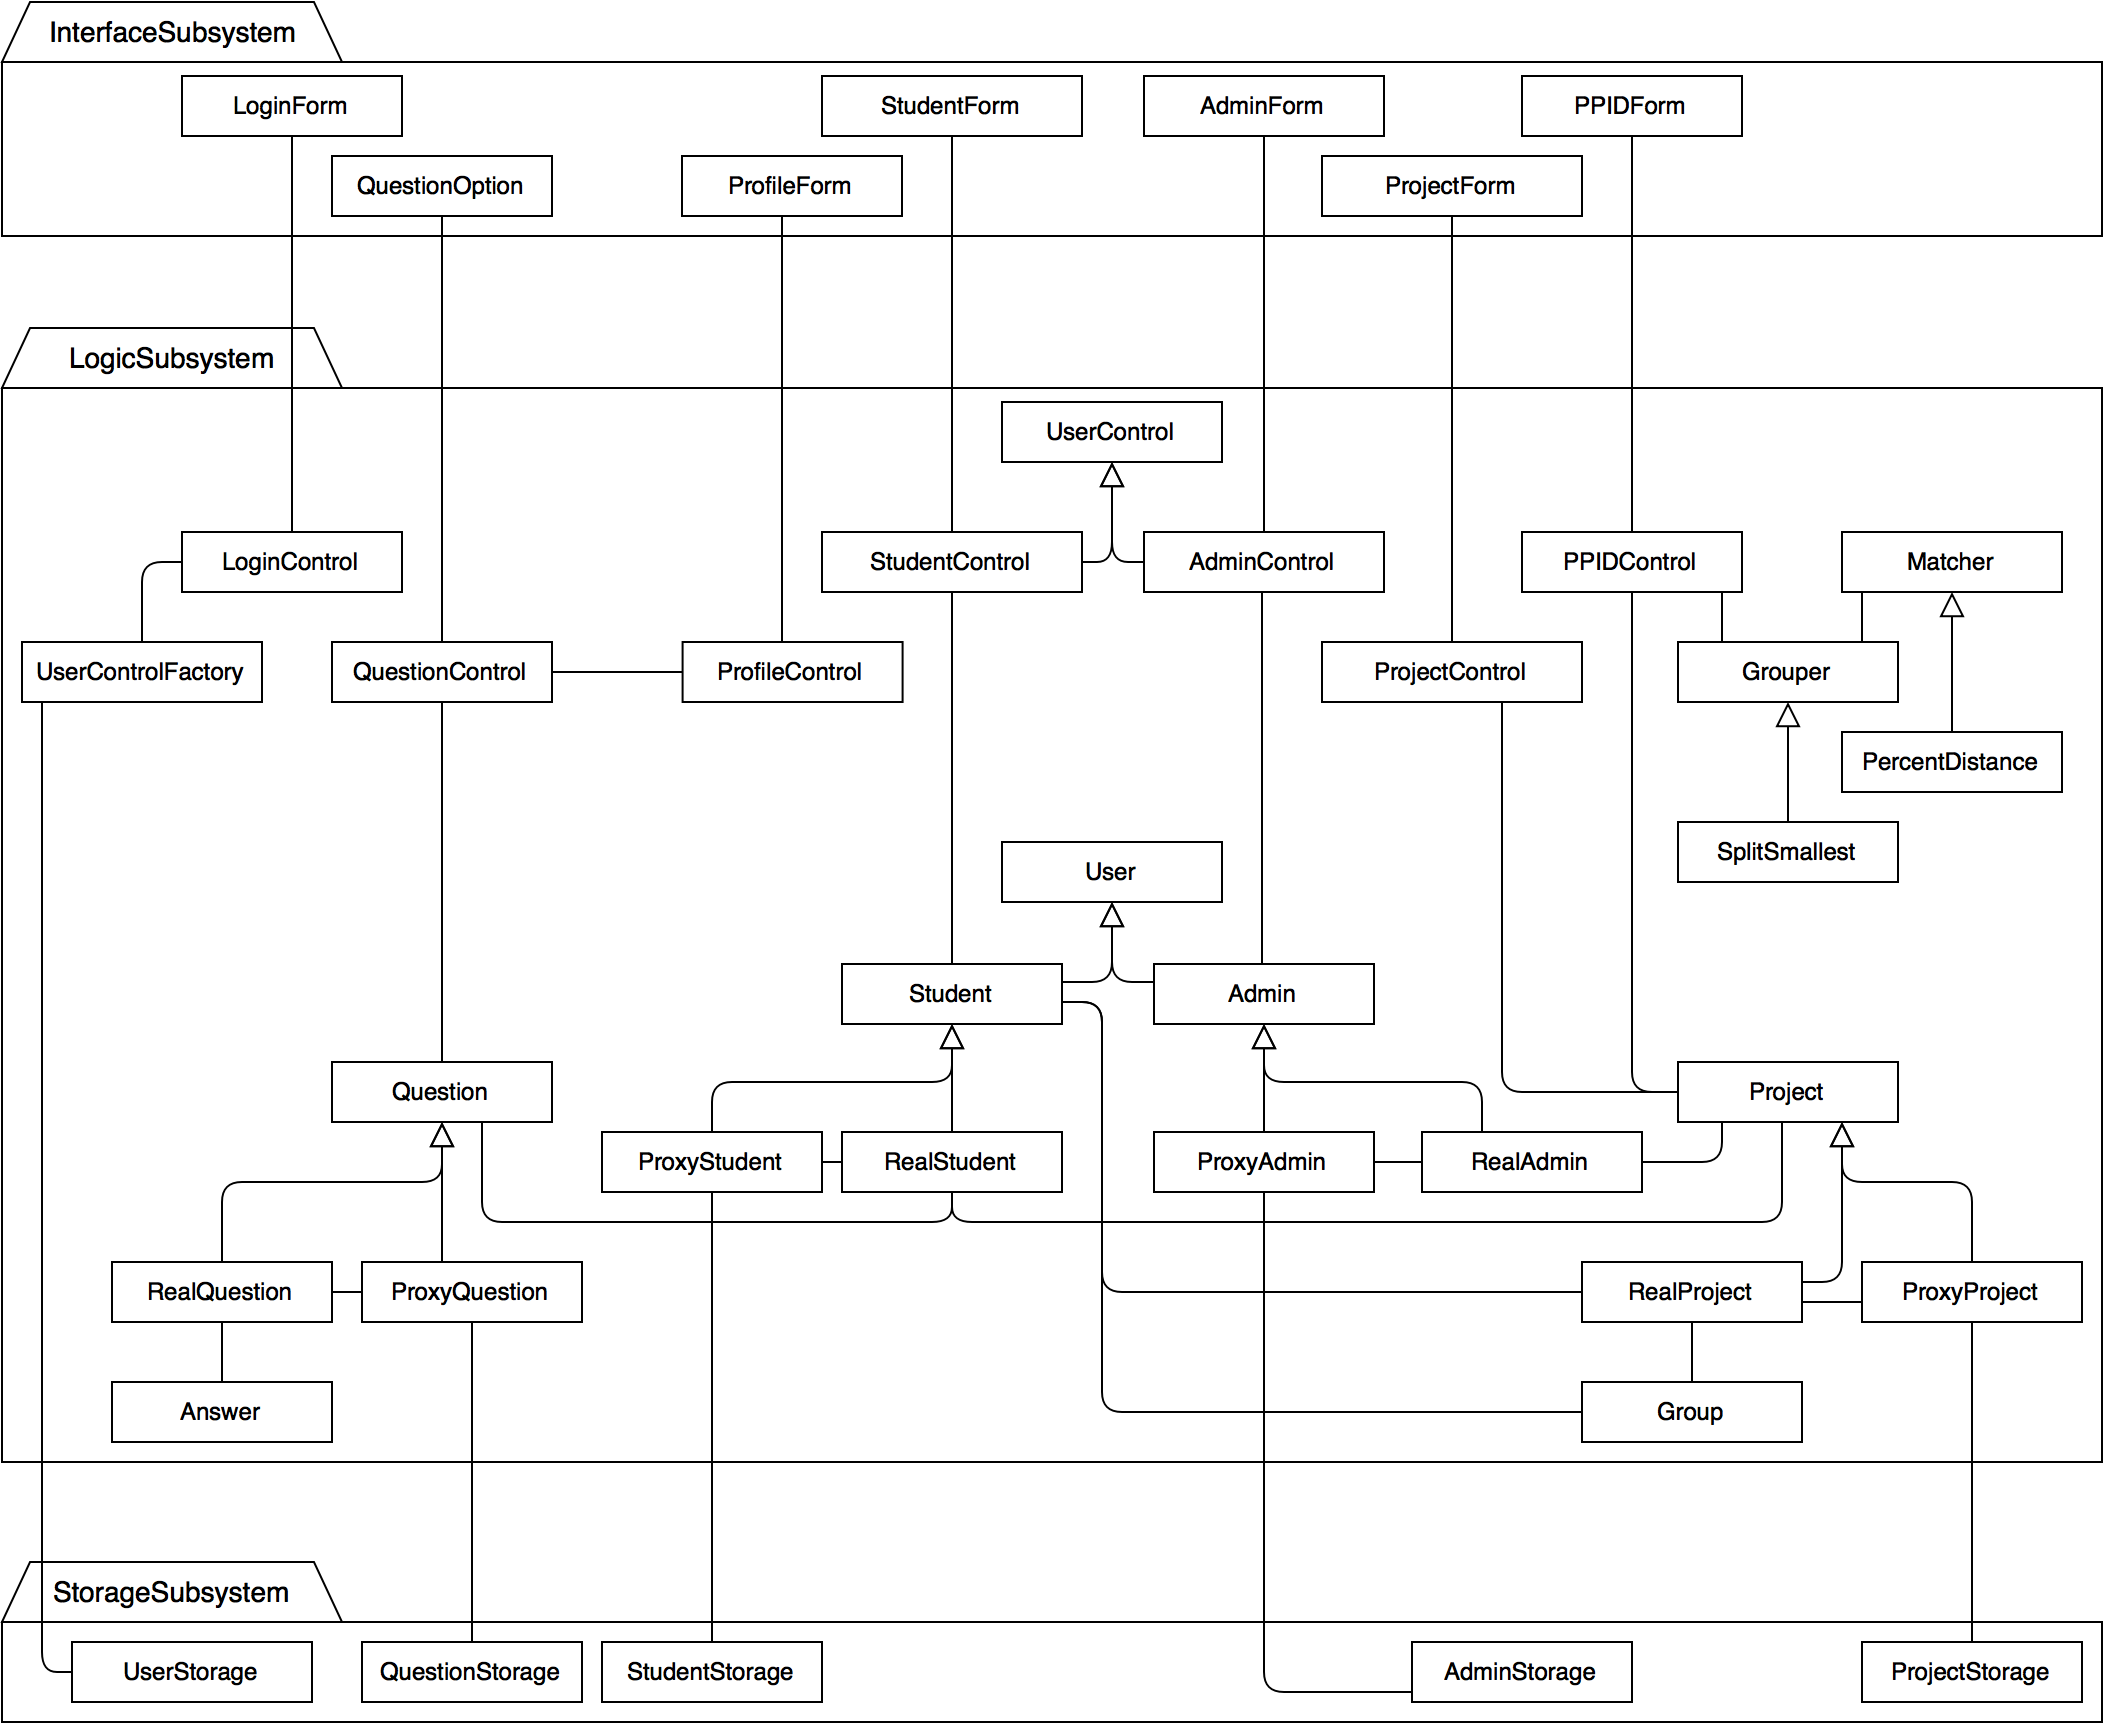
\includegraphics[scale=0.22]{imgs/d3/decomp/three-tier.png}
	\caption{Three-Tier Subsystem Decomposition}
	\figurelabel{three-tier}
\end{figure}
\subsubsection{Model-View Controller Architecture}
\subsubsection{Repository Architecture}

The Repository architectural style involves an absolutely necessary storage layer, followed by many subsystems one layer up. Essentially, this style boasts two layers, wherein the second layer would have multiple partitions. This is the architectural style that we decided to implement for our system design because of the incredibly appealing benefits: by organzing our system like this, we can achieve extremely high cohesion along with minimal coupling. This means that there are very few interdepencies between different subsystems.

\begin{figure}[H]
	\centering{}
	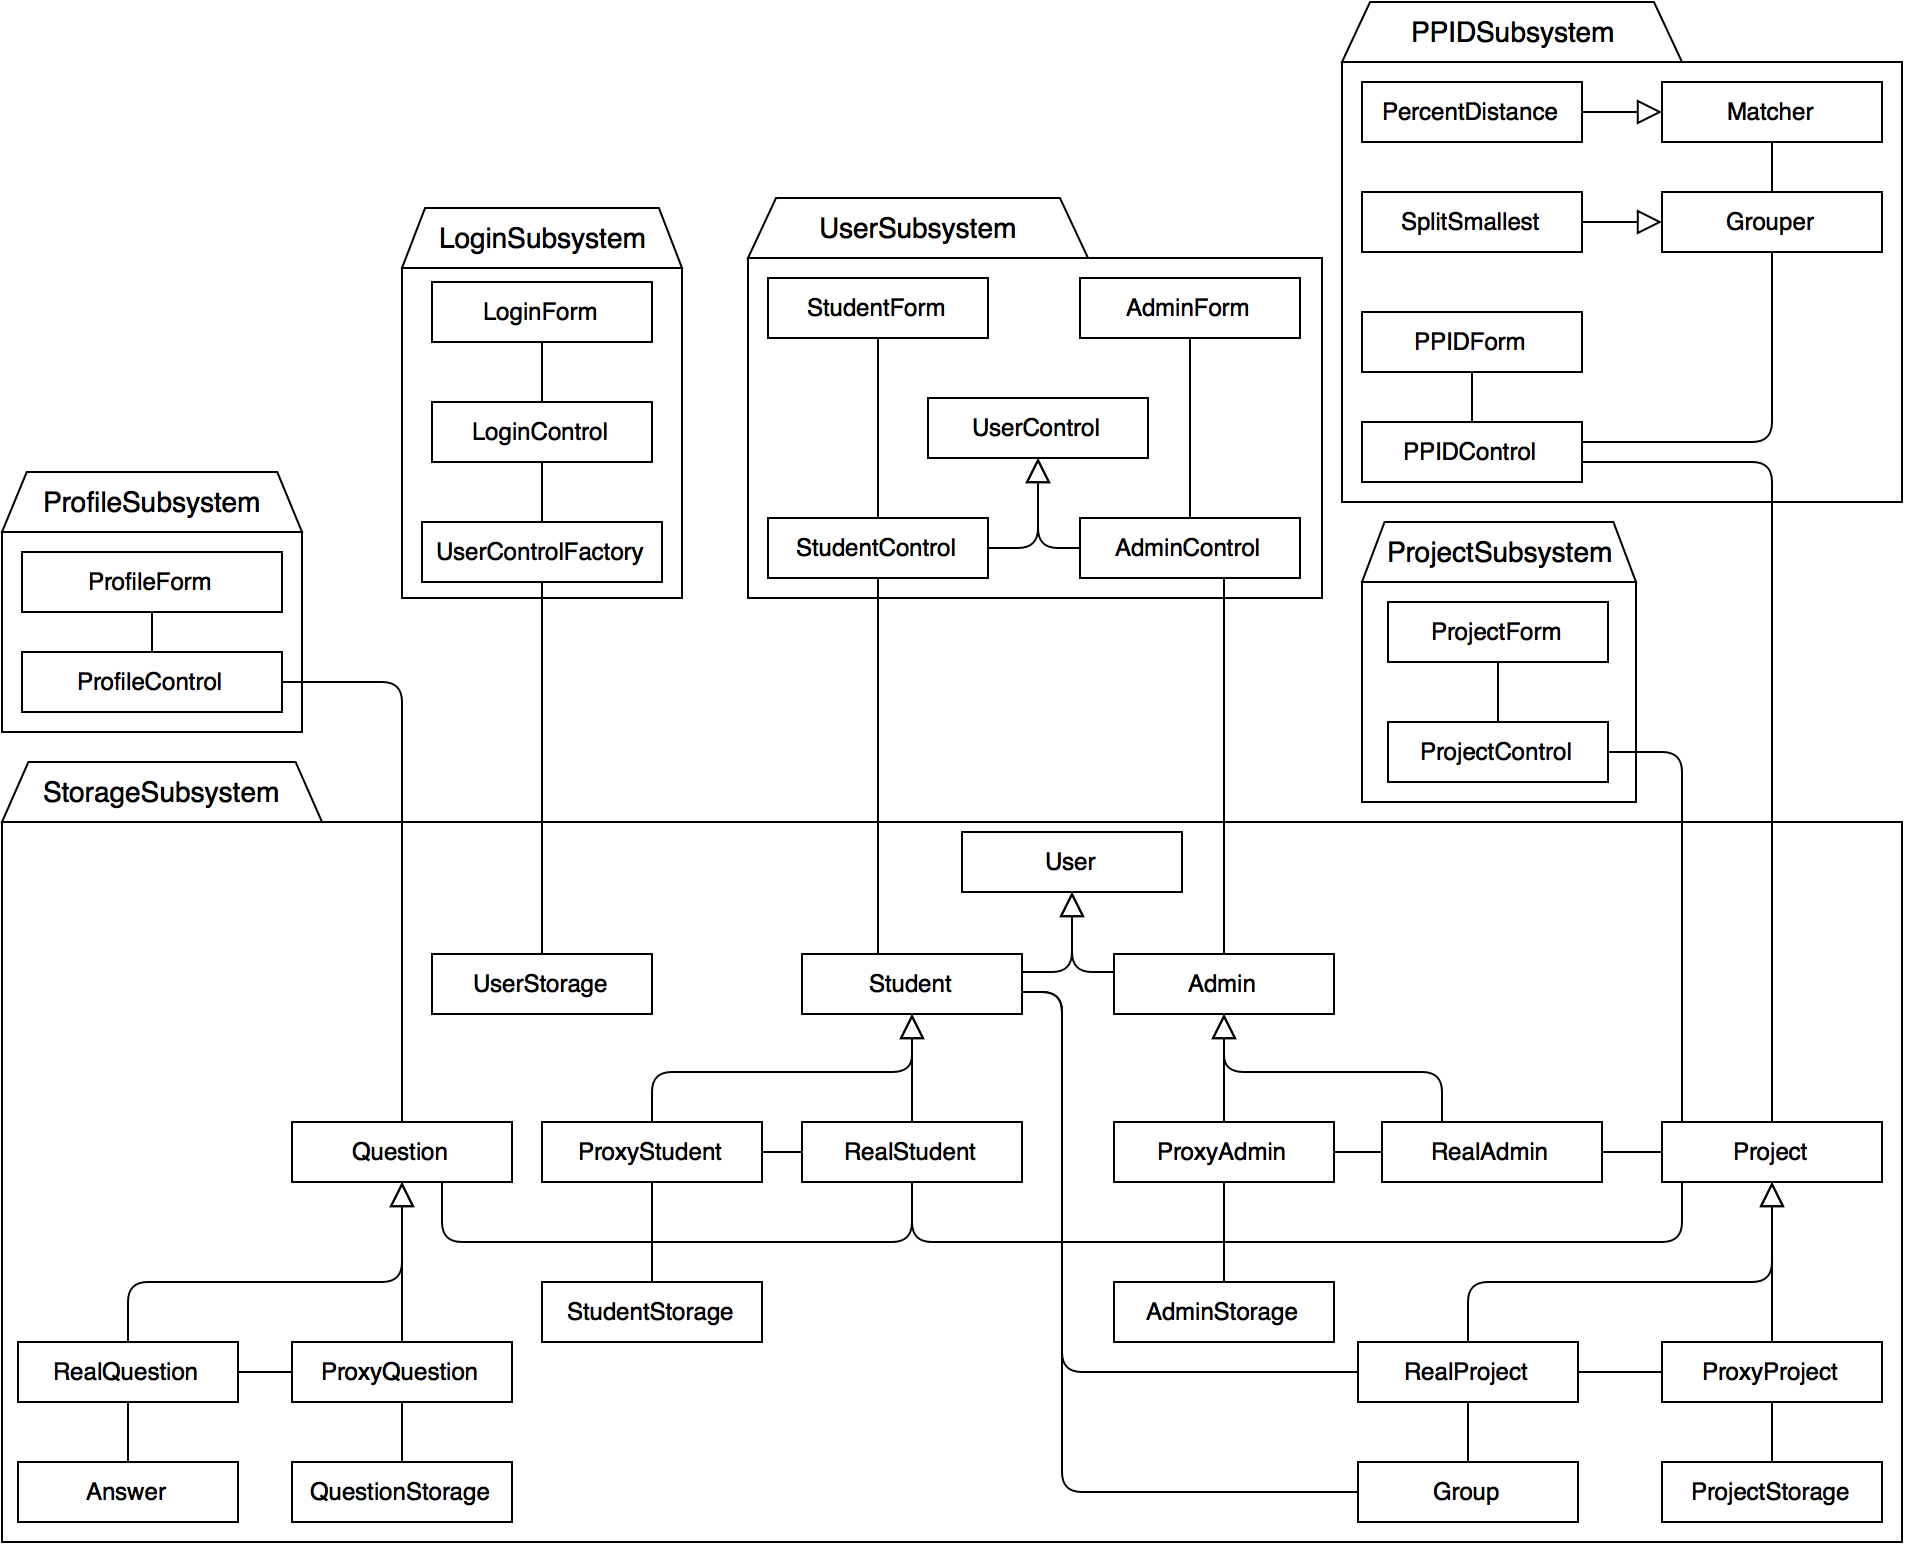
\includegraphics[scale=0.24]{imgs/d3/decomp/repository.png}
	\caption{Three-Tier Subsystem Decomposition}
	\figurelabel{three-tier}
\end{figure}
\subsection{Persistent Data Management}
\subsubsection{Overview}

To store the data for our system, a relational database is being used. Our relational database is built in the SQLite architecture. Multiple tables are used to store related information together, such as the \textit{students} table.

\begin{figure}[H]
	\centering{}
	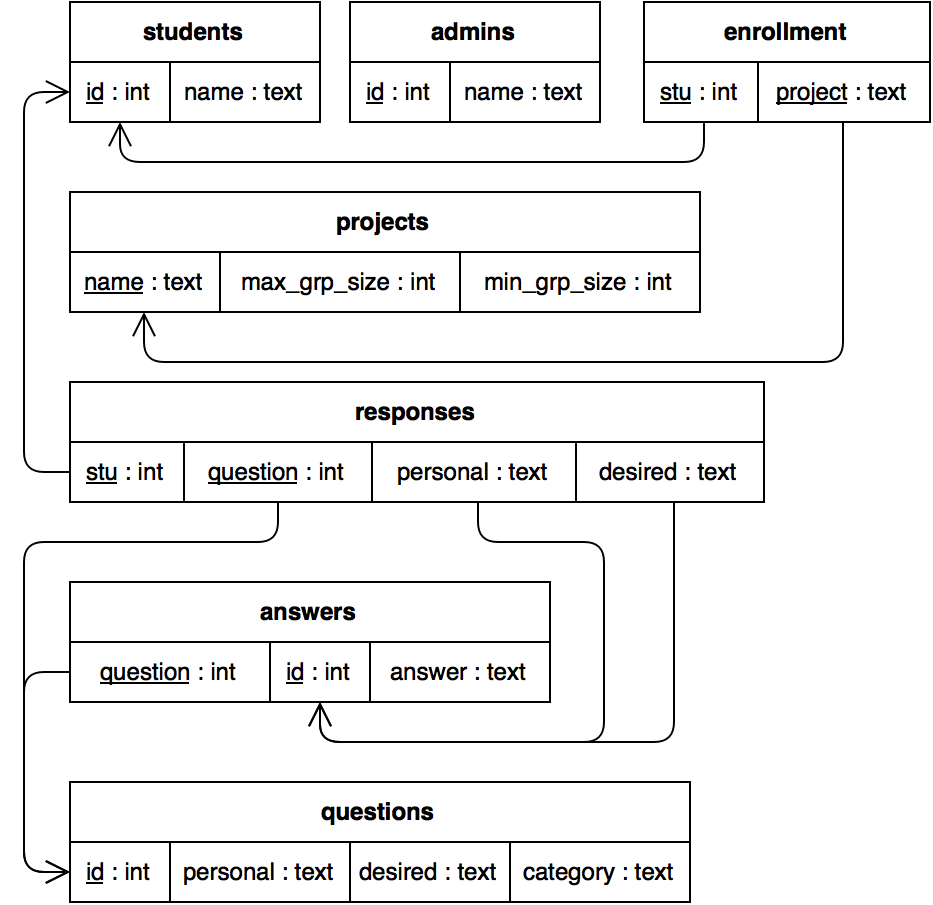
\includegraphics[scale=0.45]{imgs/d3/db/database-schema-diagram.png}
	\caption{Database Schema}
	\figurelabel{db-schema}
\end{figure}

\subsubsection*{Tables in Database}
\begin{table}[H]
	\caption{Tables in Database} \tablelabel{db-table}
	\begin{tabu} to \textwidth {l >{\it}l X}
		\tableheader{}ID & Name & Description \\
		\dtlabel{students}\dtref{students}     & students   & Stores the \textit{Student} (\cdref{student}) entity object. \\
		\dtlabel{admins}\dtref{admins}         & admins     & Stores the \textit{Admin} (\cdref{admin}) entity object. \\
		\dtlabel{projects}\dtref{projects}     & projects   & Stores the \textit{Project} (\cdref{project}) entity object. \\
		\dtlabel{enrollment}\dtref{enrollment} & enrollment & Stores the association between the \textit{Student} (\cdref{student}) 
		                                                      and \textit{Project} (\cdref{project}) entity objects, which is refers 
		                                                      to a student's enrollment into a project. \\
		\dtlabel{questions}\dtref{questions}   & questions  & Stores the \textit{Question} (\cdref{question}) entity object. \\
		\dtlabel{answers}\dtref{answers}       & answers    & Stores the \textit{Answer} (\cdref{answer}) entity object. \\
		\dtlabel{responses}\dtref{responses}   & responses  & Stores the association between the \textit{Student} (\cdref{student}) 
		                                                      and \textit{Question} (\cdref{question}) entity objects, which refers to      
		                                                      what answer a student has selected for a question. \\
	\end{tabu}
\end{table}

\begin{table}[H]
	\caption{Students Table (\dtref{students})} \tablelabel{students-table}
	\begin{tabu} to \textwidth {l l l X}
		\tableheader{}Column & Type & Constraint & Description \\
		id   & Integer & Primary Key & The unique ID given to the Student. \\
		name & Text    &             & The name of the Student. \\
	\end{tabu}
\end{table}

\begin{table}[H]
	\caption{Admins Table (\dtref{admins})} \tablelabel{admins-table}
	\begin{tabu} to \textwidth {l l l X}
		\tableheader{}Column & Type & Constraint & Description \\
		id   & Integer & Primary Key & The unique ID given to the Admin. \\
		name & Text    &             & The name of the Admin. \\
	\end{tabu}
\end{table}

\begin{table}[H]
	\caption{Projects Table (\dtref{projects})} \tablelabel{projects-table}
	\begin{tabu} to \textwidth {l l X X[3]}
		\tableheader{}Column & Type & Constraint & Description \\
		id             & Integer & Primary Key      & The unique ID given to a Project. \\
		name           & Text    & Unique,\newline 
		                           Case Insensitive & The unique name given to a Project. \\
		max\_grp\_size & Integer &                  & The maximum group size of a Project. \\
		min\_grp\_size & Integer &                  & The minimum group size of a Project. \\
	\end{tabu}
\end{table}

\begin{table}[H]
	\caption{Enrollment Table (\dtref{enrollment})} \tablelabel{enrollment-table}
	\begin{tabu} to \textwidth {l l X X[4]}
		\tableheader{}Column & Type & Constraint & Description \\
		stu     & Integer & Primary Key,\newline
		                    Foreign Key          & References \textit{id} of the \textit{students} table (\dtref{students}). \\
		project & Integer & Primary Key,\newline
		                    Foreign Key          & References \textit{id} of the \textit{projects} table (\dtref{projects}). \\
	\end{tabu}
\end{table}

\begin{table}[H]
	\caption{Questions Table (\dtref{questions})} \tablelabel{questions-table}
	\begin{tabu} to \textwidth {l l l X}
		\tableheader{}Column & Type & Constraint & Description \\
		id       & Integer & Primary Key & The unique identifier given to a Question. \\
		personal & Text    &             & Asks the Student to describe their self. \\
		desired  & Text    &             & Asks the Student to described their desired partner. \\
		category & Text    &             & The qualification category the Question belongs. \\
	\end{tabu}
\end{table}

\begin{table}[H]
	\caption{Answers Table (\dtref{answers})} \tablelabel{answers-table}
	\begin{tabu} to \textwidth {l l X X[4]}
		\tableheader{}Column & Type & Constraint & Description \\
		question & Integer & Primary Key,\newline
		                     Foreign Key          & The Question the answer belongs to. References \textit{id} of the 
		                                            \textit{questions} table. \\
		id       & Integer & Primary Key          & The unique ID given to the Answer. \\
		answer   & Text    &                      & The answer of a Question. \\
	\end{tabu}
\end{table}

\begin{table}[H]
	\caption{Responses Table (\dtref{responses})} \tablelabel{responses-table}
	\begin{tabu} to \textwidth {l l X X[4]}
		\tableheader{}Column & Type & Constraint & Description \\
		stu      & Integer & Primary Key,\newline
		                     Foreign Key          & Identifies the associated Student with the response. References \textit{id} of the 
		                                            \textit{students} table. \\
		question & Integer & Primary Key,\newline
		                     Foreign Key          & Identifies which Question the response belongs to. References \textit{question}
		                                            of the \textit{answers} table. \\
		personal & Integer & Foreign Key          & Identifies a Student's selection for their personal attribute for the given
		                                            given question. References \textit{id} of the \textit{answers} table. \\
		desired  & Integer & Foreign Key          & Identifies a Student's selection for their desired attribute for the given
		                                            given question. References \textit{id} of the \textit{answers} table. \\
	\end{tabu}
\end{table}

\subsubsection{Reasoning}
\subsubsection*{Students Table (\dtref{students})}
To ensure that ID of a \textit{Student} (\cdref{student}) is unique, the \textit{id} column is set as the primary key. This guarantees that no two IDs can be equal. As well, by having the \textit{id} column as the primary key, the speed of looking up a \textit{Student} by their ID is increased.

There isn't a constraint put on the \textit{name} column to allow for \textit{Students} with the same name to be entered into the database.

\subsubsection*{Administrator Table (\dtref{admins})}
To ensure that ID of a \textit{Admin} (\cdref{admin}) is unique, the \textit{id} column is set as the primary key. This guarantees that no two IDs can be equal. As well, by having the \textit{id} column as the primary key, the speed of looking up a \textit{Admin} by their ID is increased.

There isn't a constraint put on the \textit{name} column to allow for \textit{Admins} with the same name to be entered into the database.

\subsubsection*{Projects Table (\dtref{projects})}
Oftentimes, admins will have to create multiple projects. To assure that no duplicate projects exist, we have enforced a unique project name as the Primary Key. This assures that the admin won't confuse themselves by having several identically named projects, thus maximizing readabilit and useability. Projects also have columns storing the max and min group sizes, which are importantly distinct from one another as to allow maximum flexibility with regards to number of students enrolled in a project (for when the PPID is run).

\subsubsection*{enrollment}
Its important that each student can only enroll in each project once. To accomplish this, we have two Primary Keys - the student's unique identitier (\textit{students}.\textit{id}) and the project's unique name (\textit{projects}.\textit{name}).

\subsubsection*{questions}
- each question has unique ID so it is easy to reference 

\subsubsection*{answers}
- primary key made of foreign key to \textit{questions}.\textit{id} and \textit{id}. \\
- this allows an answer to belong to only one question. 

\subsubsection*{responses}
- using \textit{students}.\textit{id} and \textit{questions}.\textit{id}, guarantees that a student may have only one response per question.

\subsection{Design Patterns}
\subsubsection{Overview}
While organizing code with an eye to the larger picture - architectural styles - is vitally important, the smaller scale design patterns fall not far behind. Design patterns are largely independent of the architectural style insofar as nearly all design patterns can be implemented in any of the architectural patterns. They usually are used to minimize coupling across layers or to maximize cohesion across sister subsystems (partitions). This section will go over several different design patterns and explain either why we decide to use them or why we forgo their implementation. There are three main categories of design patterns that we will include in this breakdown: creational patterns, structural patterns, and behavioural patterns.
\subsubsection{Creational Patterns}
Patterns in this section affect how objects get created. 
\subsubsection*{Factory Method}
We have decided to implement this design pattern in our system. Add more here later.
\subsubsection{Structural Patterns}
\subsubsection*{Adapter}
This design pattern is ill suited to our particular system since we will be developing the entirety of our system. Since we will not need to write code that adapts between newer and older code, this pattern would be counter-intuitive.
\subsubsection*{Bridge}
\subsubsection*{Facade}
\subsubsection*{Proxy}
We have chosen to implement this design pattern in our system. By encompassing several of our entity objects in a proxy design, we can implement a `lazy' load-type system in that the system will only load the information that we directly ask for - nothing extra. This has the enormous benefit of reducing the memory footprint. The time trade-off is comparably minimal, even negligible. 
\subsubsection{Behavioural Patterns}
\subsubsection*{Command}
\subsubsection*{Observer}
\subsubsection*{Strategy}
Using this class.....................
\section{Subsystem Services}
\subsection{Overview}
\subsection{Services}

In this section, we give a list and description of each of the services that our subsystems offer. They will be divided into three separate tables - one for each of our subsystems. \sdlabel{storage}The following table encompasses all the services offered by the Proxy Subsystem (\sdref{storage}). 

\begin{table}[H]
\caption{Services Offered by the StorageSubsystem (\sdref{storage})} \tablelabel{service-sub-storage}
\begin{tabu} to \textwidth {l >{\it}l X}
	\tableheader{}ID & Service & Description\\
	\sslabel{data}\ssref{data} & Data Service & This service encompasses the operations related to getting or setting data that is being held in the persistent relational database storages. \\
\end{tabu}
\end{table}

\sdlabel{ppid}The following table showcases all the different services offered by the PPIDSubsytem (\sdref{ppid}).

\begin{table}[H]
\caption{Services Offered by PPIDSubsystem (\sdref{ppid})} \tablelabel{service-sub-ppdi}
\begin{tabu} to \textwidth {l >{\it}l X}
	\tableheader{}ID & Service & Description\\
	\sslabel{sortstudents}\ssref{sortstudents} & Student-Sorting Service & This service encompasses several operations that handle the running of the PPID algorithm, which sorts the given set of Student objects into groups.\\
\end{tabu}
\end{table}

\sdlabel{login}The following table showcases all the different services offered by the LoginSubsytem (\sdref{login}).

\begin{table}[H]
\caption{Services Offered by LoginSubsystem (\sdref{login})} \tablelabel{service-sub-login}
\begin{tabu} to \textwidth {l >{\it}l X}
	\tableheader{}ID & Service & Description\\
	\sslabel{service5}\ssref{service5} & service5 & desc\\
	\sslabel{service6}\ssref{service6} & service6 & desc\\
\end{tabu}
\end{table}

\sdlabel{profile}The following table showcases all the different services offered by the ProfileSubsytem (\sdref{profile}).

\begin{table}[H]
\caption{Services Offered by ProfileSubsystem (\sdref{profile})} \tablelabel{service-sub-profile}
\begin{tabu} to \textwidth {l >{\it}l X}
	\tableheader{}ID & Service & Description\\
	\sslabel{service5}\ssref{service5} & service5 & desc\\
	\sslabel{service6}\ssref{service6} & service6 & desc\\
\end{tabu}
\end{table}
\sdlabel{user}The following table showcases all the different services offered by the UserSubsytem (\sdref{user}).

\begin{table}[H]
\caption{Services Offered by UserSubsystem (\sdref{user})} \tablelabel{service-sub-user}
\begin{tabu} to \textwidth {l >{\it}l X}
	\tableheader{}ID & Service & Description\\
	\sslabel{service5}\ssref{service5} & service5 & desc\\
	\sslabel{service6}\ssref{service6} & service6 & desc\\
\end{tabu}
\end{table}
\sdlabel{project}The following table showcases all the different services offered by the ProjectSubsytem (\sdref{project}).

\begin{table}[H]
\caption{Services Offered by ProjectSubsystem (\sdref{project})} \tablelabel{service-sub-project}
\begin{tabu} to \textwidth {l >{\it}l X}
	\tableheader{}ID & Service & Description\\
	\sslabel{service5}\ssref{service5} & service5 & desc\\
	\sslabel{service6}\ssref{service6} & service6 & desc\\
\end{tabu}
\end{table}

\subsection{Operations}

In this section, we focus on the Operations that each of the services described in the above section offer. For added traceability, we have also included the specific class that provides each of the operations, as well as a description of each.

\begin{table}[H]
\caption{Operations Offered in Data Service (\ssref{data})} \tablelabel{operation-data}
\begin{tabu} to \textwidth {l >{\it}l l X}
	\tableheader{}ID & Operation & Class & Description\\
	\oplabel{getstuname}\opref{getstuname} & GetStudentName & ProxyStudent & desc\\
	\oplabel{getadminname}\opref{getadminname} & GetAdminName & ProxyAdmin & desc\\
	\oplabel{getprojectname}\opref{getprojectname} & GetProjectName & ProxyProject & desc\\
	\oplabel{getdesiredquestion}\opref{getdesiredquestion} & GetDesiredQuestion & ProxyQuestion & desc\\
	\oplabel{getpersonalquestion}\opref{getpersonalquestion} & GetPersonalQuestion & ProxyQuestion & desc\\
	\oplabel{getcategory}\opref{getcategory} & GetQuestionCategory & ProxyQuestion & desc\\
	\oplabel{getmaxgroupsize}\opref{getmaxgroupsize} & GetMaxGroupSize & ProxyProject & desc\\
	\oplabel{getmingroupsize}\opref{getmingroupsize} & GetMinGroupSize & ProxyProject & desc\\
\end{tabu}
\end{table}

\begin{table}[H]
\caption{Operations Offered in Student-Sorting Service (\ssref{studentsort})} \tablelabel{operation-studentsort}
\begin{tabu} to \textwidth {l >{\it}l l X}
	\tableheader{}ID & Operation & Class & Description\\
	\oplabel{operation3}\opref{operation3} & operation1 & classA & desc\\
	\oplabel{operation4}\opref{operation4} & operation2 & classB & desc\\
\end{tabu}
\end{table}

\begin{table}[H]
\caption{Operations Offered in Service3 (\ssref{service3})} \tablelabel{operation-service3}
\begin{tabu} to \textwidth {l >{\it}l l X}
	\tableheader{}ID & Operation & Class & Description\\
	\oplabel{operation5}\opref{operation5} & operation1 & classA & desc\\
	\oplabel{operation6}\opref{operation6} & operation2 & classB & desc\\
\end{tabu}
\end{table}

\begin{table}[H]
\caption{Operations Offered in Service4 (\ssref{service4})} \tablelabel{operation-service4}
\begin{tabu} to \textwidth {l >{\it}l l X}
	\tableheader{}ID & Operation & Class & Description\\
	\oplabel{operation7}\opref{operation7} & operation1 & classA & desc\\
	\oplabel{operation8}\opref{operation8} & operation2 & classB & desc\\
\end{tabu}
\end{table}

\begin{table}[H]
\caption{Operations Offered in Service5 (\ssref{service5})} \tablelabel{operation-service5}
\begin{tabu} to \textwidth {l >{\it}l l X}
	\tableheader{}ID & Operation & Class & Description\\
	\oplabel{operation9}\opref{operation9} & operation1 & classA & desc\\
	\oplabel{operation10}\opref{operation10} & operation2 & classB & desc\\
\end{tabu}
\end{table}

\section{Class Interfaces}

\begin{table}[H]
\caption{} 
\begin{tabu} to \textwidth {l >{\it}l X}
	\tableheader{}ID & Class Name & Description \\
	\cdlabel{user}\cdref{user} & User & The user class contains two attributes - the unique ID, and a name. It provides the archetype for a generic user - the defining feature being the unique identifier.\\
	\cdlabel{student}\cdref{student} & Student & The Student class contains several attributes: a unique ID, a name, both inherited from the User class, a collection of responses, and their join-status with regards to projects. Their methods revolve around the handling of their profiles, such as modifying response values. This class inherits from the User class. \\
	\cdlabel{realstudent}\cdref{realstudent} & RealStudent & The RealStudent class inherits from the Student class and contains the actual information pulled from the StudentStorage object. It is relatively hidden from the rest of the system, though the data can be accessed through the ProxyStudent object.\\
	\cdlabel{proxystudent}\cdref{proxystudent} & ProxyStudent & The ProxyStudent class also inherits from the Student class and provides a proxy or interface to the RealStudent object for the rest of the system. The idea here is to promote `lazy' loading with regards to the information stored in the RealStudent object.\\
	\cdlabel{studentstorage}\cdref{studentstorage} & StudentStorage & The StudentStorage class is a class that provides a set of methods to pull/push data related to the Student user from/to the relational database. The RealStudent object is the only object that directly interacts with this object.\\
	\cdlabel{admin}\cdref{admin} & Admin & The Admin class contains two attributes - the unique ID, and a name, both inherited from the User class - and several methods revolving around the handling of Project objects. This class inherits from the User class. \\
	\cdlabel{realadmin}\cdref{realadmin} & RealAdmin & The RealAdmin class inherits from the Admin class and contains the actual information pulled from the AdminStorage object. It is relatively hidden from the rest of the system, though the data contained can only be accessed through the ProxyAdmin object. \\
	\cdlabel{proxyadmin}\cdref{proxyadmin} & ProxyAdmin & The ProxyAdmin class also inherits from the Admin class and provides a proxy or interface to the RealAdmin object for the rest of the system. The idea here is to promote `lazy' loading with regards to the information stored in the RealAdmin object.\\
	\cdlabel{adminstorage}\cdref{adminstorage} & AdminStorage & The AdminStorage class is a class that provides a set of methods to pull/push data related to the Admin user from/to the relational database. The RealAdmin object is the only object that directly interacts with this object.\\
\end{tabu}
\end{table}

\begin{center}
\begin{tabu} to \textwidth {l >{\it}l X}
	\tableheader{}ID & Class Name & Description \\
	\cdlabel{project}\cdref{project} & Project & The Project class contains four attributes: a name, a minimum group size, a maximum group size, and a collection of Student objects. Its methods revolve around simply returning the collection of Students.\\
	\cdlabel{realproject}\cdref{realproject} & RealProject & The RealProject class inherits from the Project class and contains the actual information pulled from the ProjectStorage object. It is relatively hidden from the rest of the system, though the data can be accessed through the ProxyProject object.\\
	\cdlabel{proxyproject}\cdref{proxyproject} & ProxyProject & The ProxyProject also inherits from the Project class and provides a proxy or interface to the RealProject object for the rest of the system. The idea here is to promote `lazy' loading with regards to the information stored in the RealProject object.\\
	\cdlabel{projectstorage}\cdref{projectstorage} & ProjectStorage & The ProjectStorage class is a class that provides a set of methods to pull/push data related to Projects from/to the relational database. The RealProject object is the only object that directly interacts with this object.\\
	\cdlabel{question}\cdref{question} & Question & The Question class contains four attributes: a String representation of the questions used in the algorithm for the desired and personal versions of the questions, a unique identifier, and the category of the question. \\
	\cdlabel{realquestion}\cdref{realquestion} & RealQuestion & The RealQuestion class inherits from the Question class and contains the actual information pulled from the QuestionStorage object. It is relatively hidden from the rest of the system, though the data can be accessed through the ProxyQuestion object.\\
	\cdlabel{proxyquestion}\cdref{proxyquestion} & ProxyQuestion & The ProxyQuestion also inherits from the Question class and provides a proxy or interface to the RealQuestion object for the rest of the system. The idea here is to promote `lazy' loading with regards to the information stored in the RealQuestion object.\\
	\cdlabel{questionstorage}\cdref{questionstorage} & QuestionStorage & The QuestionStorage class is a class that provides a set of methods to pull/push data related to Questions from/to the relational database. The RealQuestion object is the only object that directly interacts with this object.\\
	\cdlabel{answer}\cdref{answer} & Answer & The Answer class contains three attributes: the question number, a unique identifier, and the set of answers. The methods this class provides revolve around simply returning the required set of answers.\\
\end{tabu}
\end{center}

\begin{center}
\begin{tabu} to \textwidth {l >{\it}l X}
	\tableheader{}ID & Class Name & Description \\
	\cdlabel{group}\cdref{group} & Group & \\
	\cdlabel{grouper}\cdref{grouper} & Grouper & \\
	\cdlabel{matcher}\cdref{matcher} & Matcher & \\
	\cdlabel{splitsmallest}\cdref{splitsmallest} & SplitSmallest & \\
	\cdlabel{percentdistance}\cdref{percentdistance} & PercentDistance & \\
	\cdlabel{ppidcontrol}\cdref{ppidcontrol} & PPIDControl & desc \\
	\cdlabel{logincontrol}\cdref{logincontrol} & LoginControl & desc \\
	\cdlabel{projectcontrol}\cdref{projectcontrol} & ProjectControl\\
\end{tabu}
\end{center}

\begin{center}
\begin{tabu} to \textwidth {l >{\it}l X}
	\tableheader{}ID & Class Name & Description \\
	\cdlabel{usercontrol}\cdref{usercontrol} & UserControl & \\
	\cdlabel{studenthomecontrol}\cdref{studenthomecontrol} & StudentHomeControl & desc \\
	\cdlabel{adminhomecontrol}\cdref{adminhomecontrol} & AdminHomeControl & desc \\
	\cdlabel{profilecontrol}\cdref{profilecontrol} & ProfileControl & desc \\
	\cdlabel{questioncontrol}\cdref{questioncontrol} & QuestionControl & desc \\
	\cdlabel{questionscontrol}\cdref{questionscontrol} & QuestionsControl & desc \\
	\cdlabel{userconfact}\cdref{userconfact} & UserControlFactory & \\
	\cdlabel{userstorage}\cdref{userstorage} & UserStorage & \\
	\cdlabel{loginform}\cdref{loginform} & LoginForm & \\

\end{tabu}
\end{center}

\begin{center}
\begin{tabu} to \textwidth {l >{\it}l X}
	\tableheader{}ID & Class Name & Description \\
	\cdlabel{questionsform}\cdref{questionsform} & QuestionsForm & \\
	\cdlabel{questionoption}\cdref{questionoption} & QuestionOption & \\
	\cdlabel{profileform}\cdref{profileform} & ProfileForm & \\
	\cdlabel{studentform}\cdref{studentform} & StudentForm & \\
	\cdlabel{adminform}\cdref{adminform} & AdminForm & \\
	\cdlabel{projectform}\cdref{projectform} & ProjectForm & \\
	\cdlabel{ppidform}\cdref{ppidform} & PPIDForm & \\
\end{tabu}
\end{center}

\end{document}
